% Created 2017-05-17 Wed 09:33
% Intended LaTeX compiler: pdflatex
\documentclass[a4paper,11pt]{article}
\usepackage[utf8]{inputenc}
\usepackage[T1]{fontenc}
\usepackage{graphicx}
\usepackage{grffile}
\usepackage{longtable}
\usepackage{wrapfig}
\usepackage{rotating}
\usepackage[normalem]{ulem}
\usepackage{amsmath}
\usepackage{textcomp}
\usepackage{amssymb}
\usepackage{capt-of}
\usepackage{hyperref}
\usepackage[margin=1.2in]{geometry}
\usepackage{setspace}
\onehalfspacing
\usepackage{parskip}
\usepackage{amsthm}
\usepackage{amsmath}
\usepackage{mathtools}
\usepackage{hyperref}
\usepackage{graphicx}
\usepackage{tabularx}
\usepackage{booktabs}
\usepackage{color}
\usepackage{caption}
\usepackage{subcaption}
\hypersetup{colorlinks,citecolor=black,filecolor=black,linkcolor=black,urlcolor=black}
\newtheorem{mydef}{Definition}
\newtheorem{mythm}{Theorem}
\newcommand{\dx}{\mathrm{d}}
\newcommand{\var}{\mathrm{Var}}
\newcommand{\cov}{\mathrm{Cov}}
\newcommand{\corr}{\mathrm{Corr}}
\newcommand{\pr}{\mathrm{Pr}}
\newcommand{\rarrowd}[1]{\xrightarrow{\text{ \textit #1 }}}
\DeclareMathOperator*{\plim}{plim}
\newcommand{\plimn}{\plim_{n \rightarrow \infty}}
\setcounter{secnumdepth}{2}
\author{Zheng Tian}
\date{}
\title{Lecture 10: Nonlinear Regression Functions}
\hypersetup{
 pdfauthor={Zheng Tian},
 pdftitle={Lecture 10: Nonlinear Regression Functions},
 pdfkeywords={},
 pdfsubject={},
 pdfcreator={Emacs 25.1.1 (Org mode 9.0.3)}, 
 pdflang={English}}
\begin{document}

\maketitle
\setcounter{tocdepth}{1}
\tableofcontents


\section{Introduction}
\label{sec:orgc909103}
\subsection{Overview}
\label{sec:orga62771c}
In the previous lectures, the population regression function is
assumed to be linear. In other words, the slope of the population
regression function was constant, so the effect on Y of a unit change
in X does not itself depend on the value of X, neither on other
independent variables. In some cases, the linearity cannot capture the
feature of the data and may also contradict with economic theories or
common sense.

This lecture introduces nonlinear population regression
functions that are nonlinear with respect to
the regressors but linear with respect to the parameters. Such
regression models can still be considered as being "linear" due to the
linearity in the parameters so that they can be estimated using the
OLS method we have known. Specifically, we will introduce three types
of nonlinear regression functions, the polynomial function, the
logarithmic function, and the function with the interaction terms
consisting of two independent variables.

Since these types of models can be estimated using the OLS, the
estimation and inference are not the foci of this lecture. Instead, we
put emphasis on the correct interpretation of the coefficients in each
type of models.

\subsection{Reading materials}
\label{sec:org60992b1}
\begin{itemize}
\item Chapter 8 in \emph{Introduction to Econometrics} by Stock and Watson.
\end{itemize}


\section{A General Strategy For Modeling Nonlinear Regression Functions}
\label{sec:org9f1ce83}

\subsection{Test Scores and district income}
\label{sec:orgb9807ea}

In the application of California elementary schools, we know that test
scores can be determined by average district income, along with
student-teacher ratios that we have included in regression. For
simplicity, let's just consider the relationship between test scores
and district income using a scatterplot. As shown in Figure
\ref{fig:org0767477}, test scores and district income are indeed
positively correlated, with a correlation coefficient of 0.71.

\begin{figure}[htbp]
\centering
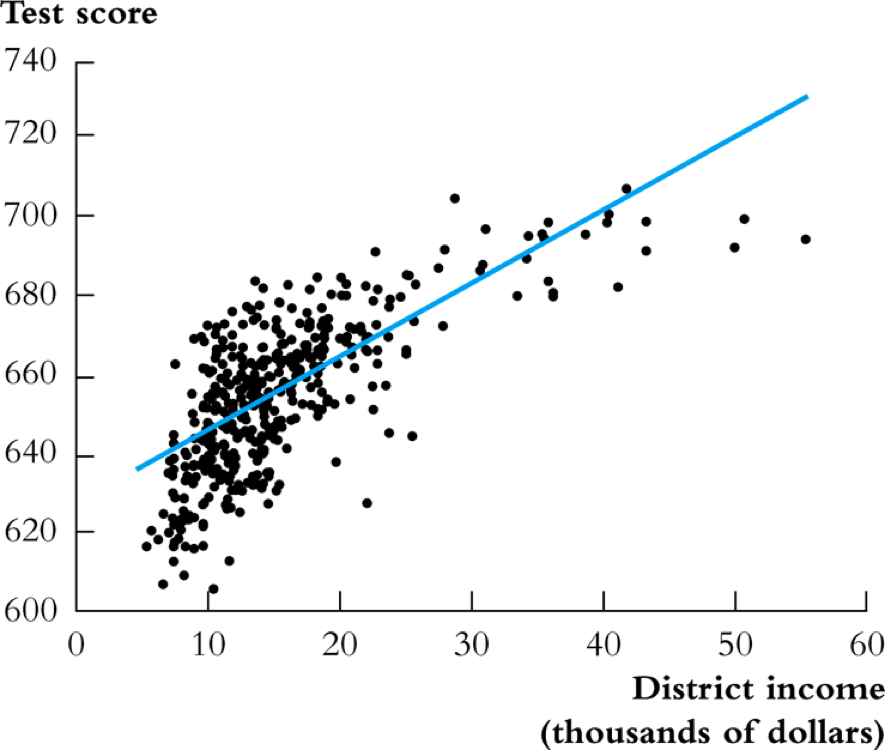
\includegraphics[width=0.75\textwidth]{img/fig-8-2.png}
\caption{\label{fig:org0767477}
Scatterplot of test score vs district income and a linear regression line}
\end{figure}

\subsubsection*{How does a simple linear regression model fit the data?}
\label{sec:org229af95}

We estimate a simple linear regression model
\[TestScore = \beta_0 + \beta_1 Income + u\]

The sample regression line is superimposed on the
scatterplot. However, we can observe some problems of using the linear
regression line to fit the data

\begin{itemize}
\item Data points are below the regression line when income is very
low (under \$10,000) or very high (over \$40,000), and are above the
line when income is between \$15,000 and \$30,000.
\item The scatterplot may imply a curvature in the relationship between
test scores and income. That is, a unit increase in income may have
larger effect on test scores when income is very low than when
income is very high.
\item The linear regression line cannot capture the curvature because the
effect of district income on test scores is constant over all the
range of income since \(\Delta TestScore / \Delta Income = \beta_1\)
is constant.
\end{itemize}

\subsubsection*{Estimate a quadratic regression model}
\label{sec:org4d5b933}

Instead of estimating a linear regression model, we can set up a
quadratic regression model as
\begin{equation}
\label{eq:quadratic-testscore}
TestScore = \beta_0 + \beta_1 Income + \beta_2 Income^2 + u
\end{equation}

\begin{itemize}
\item This model is nonlinear, specifically quadratic, with respect to
\(Income\) because we include the squared income.
\item The population regression function is
\[E(TestScore | Income) = \beta_0 + \beta_1 Income + \beta_2 Income^2\]
\item But it is linear with respect to \(\beta\). So we can still use the
OLS estimation method to estimate the model, and use \(R^2\), t and F
statistics for inference as we do in multiple regression. We simply
treat \(Income^2\) as another regressor in a multiple regression model.
\item The quadratic regression line is added onto the scatterplot, which
fits the points better than the linear regression line, as shown in
Figure \ref{fig:org46f11e9}.

\begin{figure}[htbp]
\centering
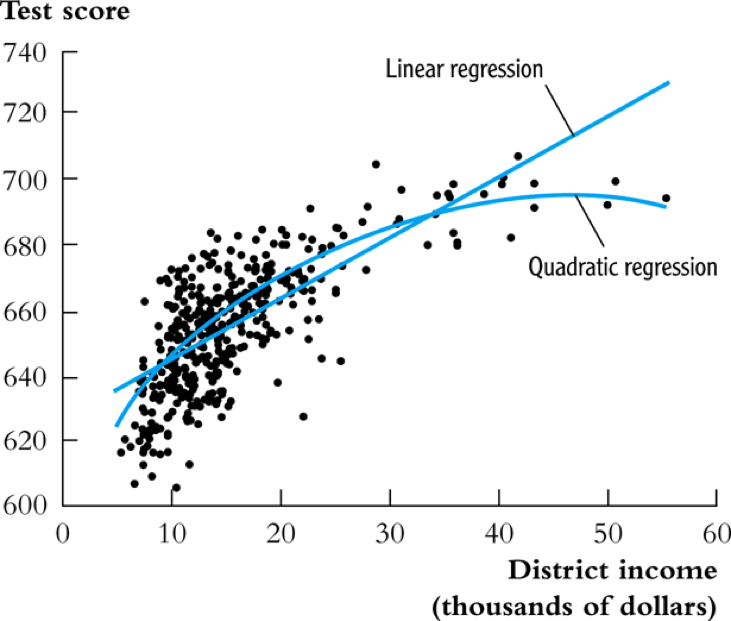
\includegraphics[width=0.75\textwidth]{img/fig-8-3.png}
\caption{\label{fig:org46f11e9}
Scatterplot of test score vs district income and a quadratic regression line}
\end{figure}
\end{itemize}


\subsection{A general formula for a nonlinear population regression function}
\label{sec:org1988d9d}

A general nonlinear regression model is
\begin{equation}
\label{eq:nl-general}
Y_i = f(X_{i1}, X_{i2}, \ldots, X_{ik}; \beta_1, \beta_2, \ldots, \beta_m) + u_i
\end{equation}

where \(f(X_{i1}, X_{i2}, \ldots, X_{ik}; \beta_1, \beta_2, \ldots,
\beta_m)\) is the \textbf{population nonlinear regression function}. Note that
the number of regressors and the number of parameters are not
necessarily equal in the nonlinear regression model.

We can use \(\mathbf{X}_i = (X_{i1}, \ldots, X_{ik})\) to represent all
regressors for the i\(^{\text{th}}\) observation, and use
\(\boldsymbol{\beta}=(\beta_1, \beta_2, \ldots, \beta_m)\) to represent
the parameters to be estimated. Then, the nonlinear regression model
in Equation (\ref{eq:nl-general}) can be re-written as

\begin{equation}
\label{eq:nl-general-mat}
Y_i = f(\mathbf{X}_i; \boldsymbol{\beta}) + u_i
\end{equation}

In this lecture, we focus on the nonlinear regression models
such that \(f(\cdot)\) is nonlinear with \(\mathbf{X}_i\) but linear with
\(\boldsymbol{\beta}\). So this type of models are also consider as
being "linear" and estimated by the OLS method.


\subsection{The effect on \(Y\) of a change in a regressor}
\label{sec:orgafbe39c}

For the general nonlinear model in Equation (\ref{eq:nl-general}), the
effect on \(Y\) of a change in one regressor, say \(X_1\), holding other
things constant, can be computed as
\begin{equation}
\label{eq:nl-gen-effect}
\Delta Y = f(X_1 + \Delta X_1, X_2, \ldots, X_k; \boldsymbol{\beta}) - f(X_1, X_2, \ldots, X_k; \boldsymbol{\beta})
\end{equation}
When \(X_1\) and \(Y\) are continuous variables and \(f(\cdot)\) is
differentiable, the marginal effect of \(X_1\) is the partial derivative
of \(f\) with respect to \(X_1\), that is, holding other things constant
\[ \mathrm{d}Y = \frac{\partial f(X_1, \ldots, X_k;
\boldsymbol{\beta})}{\partial X_i} \mathrm{d} X_i \]
because \(\mathrm{d}X_j = 0\) for \(j \neq i\). 


\subsection{Application to test scores and income}
\label{sec:orgb8168dd}

We estimate the quadratic regression model for test scores and
district income (Equation \ref{eq:quadratic-testscore}) by OLS,
resulting in the following
\begin{equation}
\label{eq:tsr-income2}
\widehat{TestScore} = \underset{\displaystyle (2.9)}{607.3} +
\underset{\displaystyle (0.27)}{3.85}Income - \underset{\displaystyle (0.0048)}{0.0423}Income^2,\, \bar{R}^2 = 0.554
\end{equation}

We can test whether the squared income has a significant
coefficient. That is, we test \(H_0:\, \beta_2 = 0 \text{ vs. } H_1:\,
\beta_2 \neq 0\). In other words, we test the quadratic regression mode
against the linear regression model. For this two-sided test, we can
as usual compute the t-statistic
\[ t = \frac{-0.0423}{0.0048} = -8.81 > -1.96 \]

Thus, we can reject the null at the 1\%, 5\% and 10\% significance levels.

From Equation (\ref{eq:tsr-income2}), we can compute the effect of
change in district average income on test scores.

\subsubsection*{A change in income from \$10 thousand to \$20 thousand}
\label{sec:org38d83e3}
\begin{equation*}
\begin{split}
\Delta \hat{Y} &= \hat{\beta}_0 + \hat{\beta}_1 \times 11 + \hat{\beta}_2 \times 11^2 - (\hat{\beta}_0 + \hat{\beta}_1 \times 10 + \hat{\beta}_2 \times 10^2) \\
&= \hat{\beta}_1 (11 - 10) + \hat{\beta}_2(11^2 - 10^2) \\
& = 3.85 - 0.0423 \times 21 = 2.96
\end{split}
\end{equation*}
Thus, the predicted difference in test scores between a district with
average income of \$11,000 and one with average income of \$10,000 is
2.96 points.

\subsubsection*{A change in income from \$40 thousand to \$41 thousand}
\label{sec:org2f9d9fb}
\begin{equation*}
\begin{split}
\Delta \hat{Y} &= \hat{\beta}_0 + \hat{\beta}_1 \times 41 + \hat{\beta}_2 \times 41^2 - (\hat{\beta}_0 + \hat{\beta}_1 \times 40 + \hat{\beta}_2 \times 40^2) \\
&= \hat{\beta}_1 (41 - 40) + \hat{\beta}_2(41^2 - 40^2) \\
& = 3.85 - 0.0423 \times 81 = 0.42
\end{split}
\end{equation*}
Thus, the predicted difference in test scores between a district with
average income of \$41,000 and one with average income of \$40,000 is
0.42 points. Thus, a change of income of \$1,000 is associated with a
larger change in predicted test scores if the initial income is
\$10,000 than if it is \$40,000.


\subsection{A general approach to modeling nonlinearities using multiple regression}
\label{sec:orgd043fd6}
\begin{enumerate}
\item Identify a possible nonlinear relationship.
\begin{itemize}
\item Economic theory
\item Scatterplots
\item Your judgment and experts' opinions
\end{itemize}
\item Specify a nonlinear function and estimate its parameters by OLS.
\begin{itemize}
\item The OLS estimation and inference techniques can be used as usual
when the regression function is linear with respect to \(\beta\).
\end{itemize}
\item Determine whether the nonlinear model can improve a linear model
\begin{itemize}
\item Use t- and/or F-statistics to test the null hypothesis that the
population regression function is linear against the alternative
that it is nonlinear.
\end{itemize}
\item Plot the estimated nonlinear regression function.
\item Compute the effect on \emph{Y} of a change in \emph{X} and interpret the
results.
\end{enumerate}


\section{Nonlinear functions of a single independent variable}
\label{sec:org539af9c}
\subsection{Polynomials}
\label{sec:org1b44132}
\subsubsection*{A polynomial regression model of degree r}
\label{sec:orgbb8ed1c}
\begin{equation}
\label{eq:poly-r}
Y_i = \beta_0 + \beta_1 X_i + \beta_2 X_i^2 + \cdots + \beta_r X_i^r + u_i
\end{equation}
\begin{itemize}
\item \(r = 2\): a \textbf{quadratic} regression model
\item \(r = 3\): a \textbf{cubic} regression model
\item A polynomial regression model is just regression of \(Y_i\) on
regressors \(X_i, X_i^2, \ldots, X_i^r\). So use the OLS method to
estimate \(\beta_1, \beta_2, \ldots, \beta_r\).
\end{itemize}

\subsubsection*{Testing the null hypothesis that the population regression function is linear}
\label{sec:org95d6325}
\[ H_0:\, \beta_2 = 0, \beta_3 = 0, ..., \beta_r = 0 \text{ vs. }
H_1:\, \text{ at least one } \beta_j \neq 0, j = 2, \ldots, r \]
\begin{itemize}
\item Use F statistic to test this joint hypothesis. The number of
restriction is \(q = r-1\).
\end{itemize}


\subsubsection*{What is \(\Delta Y / \Delta X\) in a polynomial regression model?}
\label{sec:org8546c12}

\begin{itemize}
\item Consider a cubic model and continuous \(X\) and \(Y\)
\[Y = \beta_0 + \beta_1 X + \beta_2 X^2 + \beta_3 X^3 + u\]
\item Then, we can calculate
\[\frac{\dx Y}{\dx X} = \beta_1 + 2\beta_2 X + 3\beta_3 X^2 \]
\item The effect of a unit change in \(X\) on \(Y\) depends on the value of
\(X\) at evaluation.
\end{itemize}

\subsubsection*{Which degree polynomial should I use?}
\label{sec:orgbc950fd}
\begin{itemize}
\item Balance a trade-off between flexibility and statistical precision.
\begin{itemize}
\item Flexibility. Relate Y to X in more complicated way than simple
linear regression.
\item Statistical precision. \(X, X^2, X^3, \ldots\) are correlate so
that there is the problem of imperfect multicollinearity.
\end{itemize}
\item Follow a sequential hypothesis testing procedure
\begin{enumerate}
\item Pick a maximum value of \(r\) and estimate the polynomial
regression for that \(r\).
\item Use the t-statistic to test the hypothesis that the coefficient
on \(X^r\) is zero. If you reject this hypothesis, then \(X^r\)
belongs in the regression, so use the polynomial of degree \(r\).
\item If you do not reject \(\beta_j = 0\) in step 2, eliminate \(X^r\)
from the regression and estimate a polynomial regression of
degree \(r-1\). Test whether the coefficient on \(X^{r-1}\) is
zero. If you reject, use the polynomial of degree \(r-1\).
\item If you do not reject \(\beta_{r-1} = 0\) in step 3, continue this
procedure until the coefficient on the highest power in your
polynomial is statistically significant.
\end{enumerate}
\item Quite often, we use a maximum degree of 2, 3, or 4.
\end{itemize}

\subsubsection*{Application to district income and test scores}
\label{sec:orgb540783}
We estimate a cubic regression model relating test scores to district
income as follows
\begin{equation*}
\widehat{TestScore} = \underset{\displaystyle (5.1)}{600.1} 
                    + \underset{\displaystyle (0.71)}{5.02} Income
                    - \underset{\displaystyle (0.029)}{0.096} Income^2 
                    + \underset{\displaystyle (0.00035)}{0.00069} Income^3, \hat{R}^2 = 0.555 
\end{equation*}

\begin{itemize}
\item Test whether it is a cubic model. We can test the null \(H_0: \beta_3
  = 0\) using the t-statistic, which is 1.97 so that we can reject the
null at the 5\% level but fail to reject the null at the 1\% level.
\item Test whether it is a nonlinear model. In this case, we test the null
\(H_0: \beta_2 = \beta_3 = 0\) using the F-statistic, which is 37.7
with the p-value less than 0.01\% so that we reject the null at the
1\% level.
\item Interpretation of coefficients. The coefficients in polynomial
regressions do not have a simple interpretation. The best way to
interpret is to plot the estimated regression function and calculate
the estimated effect on Y associated with a change in X for one or
more values of X.
\end{itemize}


\subsection{Logarithms}
\label{sec:orgb057295}
\subsubsection*{A natural logarithmic function \(y = \ln(x)\)}
\label{sec:orgf2130c7}
\begin{itemize}
\item Properties of \(\ln(x)\)
\begin{gather*}
\ln(1/x) = -\ln(x),\, \ln(ax) = \ln(a) + \ln(x) \\
\ln(x/a) = \ln(x) - \ln(a),\, \text{ and } \ln(x^a) = a\ln(x)
\end{gather*}

\item The derivative of \(\ln(x)\) is
\[ \frac{\dx \ln(x)}{\dx x} = \lim_{\Delta x \rightarrow 0}
  \frac{\ln(x + \Delta x) - \ln(x)}{\Delta x} = \frac{1}{x}\,\text{.} \]
It follows that \(\dx \ln(x) = \dx x / x\), representing the percentage
change in \(x\).

\item We can also denote the "percentage-change" form using the \(\Delta\)
operator, that is,
\[ \ln(x + \Delta x) - \ln(x) \approx \frac{\Delta x}{x} \text{ when
  } \Delta x \text{ is small.} \]

We can reach the above equation by the Taylor expansion of \(\ln(x +
  \Delta x)\) at \(x\), which is
\begin{align*}
\ln(x + \Delta x) &= \ln(x) + \frac{\dx \ln(x)}{\dx} (x + \Delta x - x) + \frac{1}{2!}\frac{\dx^2 \ln(x)}{\dx x^2}(x + \Delta x - x)^2 + \cdots \\
&= \ln(x) + \frac{\Delta x}{x} -\frac{\Delta x^2}{2x^2} + \cdots
\end{align*}
When \(\Delta x\) is very small, we can omit the terms with \(\Delta
  x^2, \Delta x^3\), etc. Thus, we have \(\ln(x + \Delta x) - \ln(x)
  \approx \frac{\Delta x}{x}\) when \(\Delta x\) is small.
\end{itemize}

\subsubsection*{The three logarithmic regression models}
\label{sec:org3aa34c8}
There are three types of logarithmic regression models. Differences in
logarithmic transformation of \(X\) and/or \(Y\) lead to differences in
interpretation of the coefficient.

\begin{itemize}
\item \textbf{Case I: linear-log model}
\label{sec:orgc0bf9ad}

In this case \(X\) is in logarithms, \(Y\) is not.
\begin{equation}
\label{eq:linear-log}
Y_i = \beta_0 + \beta_1 \ln(X_i) + u_i, i = 1, \ldots, n
\end{equation}
In the linear-log model, a 1\% change in \(X\) is associated with a
change in \(Y\) of 0.01\(\beta_{\text{1}}\) because
\[ \Delta Y = \beta_1 \ln(X + \Delta X) - \beta_1 \ln(X) \approx
\beta_1 \frac{\Delta X}{X} \]
If \(X\) changes by 1\%, then \(\Delta X/X = 0.01\) and \(\Delta Y =
0.01\beta_1\). Using the derivative of \(ln(x)\), we can easily see that
\(\beta_1 = \dx Y/\dx \ln(X) = \dx Y / (\dx X/X)\).

\emph{e.g.} Suppose that we have the estimated model as
\[\widehat{TestScore} = 557.8 + 36.42\ln(Income)\]
Then it implies that 1\% increase in average district income results in an
increase in test scores by \(0.01 \times 36.42 = 0.36\) point.

\begin{figure}[htbp]
\centering
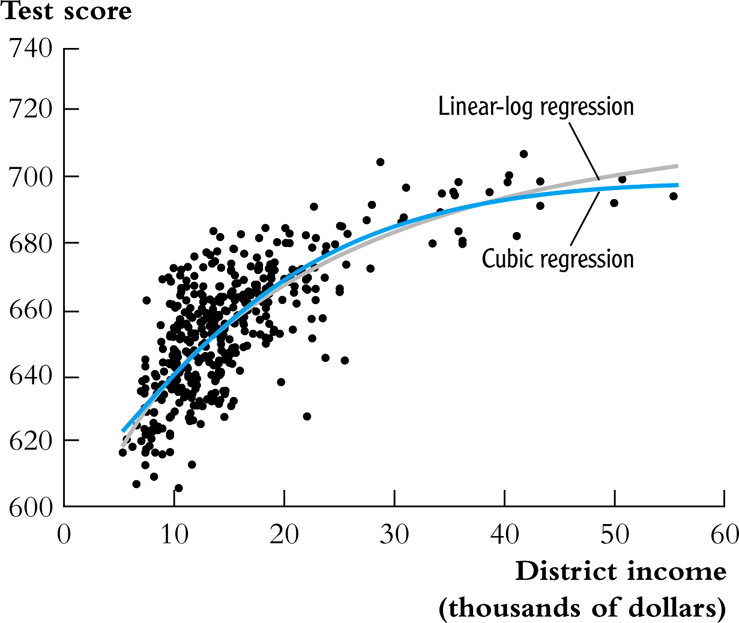
\includegraphics[width=0.65\textwidth]{img/fig-8-5.png}
\caption{\label{fig:org3d8b02e}
The linear-log and cubic regression function}
\end{figure}

\item \textbf{Case II: log-linear model}
\label{sec:org3ad0a4f}

In this case \(Y\) is in logarithms, \(X\)
is not.
\begin{equation}
\label{eq:log-linear}
\ln(Y_i) = \beta_0 + \beta_1 X_i + u_i
\end{equation}
In the log-linear model, a one-unit change in \(X\) is associated
with a \(100 \times \beta_1\%\) change in \(Y\) because
\begin{equation*}
\frac{\Delta Y}{Y} \approx \ln(Y + \Delta Y) - \ln(Y) = \beta_1 \Delta X
\end{equation*}
If \(\Delta X = 1\), then \(\Delta Y / Y = \beta_1\). Expressed in
percentage, we say that \(Y\) change by \(100\beta_1\%\). With the
derivative, \(\beta_1 = \dx \ln(Y) / \dx X = (\dx Y/Y) / X\).

\emph{e.g.} In a regression of earnings on age, we have the estimated
model as
\[ \widehat{\ln(Earnings)} = 2.805 + 0.0087Age \]
So in this regression, earnings are predicted to increase by
0.87\% for each additional year of age.

\item \textbf{Case III: log-log model}
\label{sec:org0e11cec}

In this case both \(X\) and \(Y\) are in
logarithms.
\begin{equation}
\label{eq:log-log}
\ln(Y_i) = \beta_0 + \beta_1 \ln(X_i) + u_i
\end{equation}
In the log-log model, 1\% change in \(X\) is associated with a
\(\beta\)\_1\% change in \(Y\) because
\[ \frac{\Delta Y}{Y} \approx \ln(Y + \Delta Y) - \ln(Y) =
\beta_1 (\ln(X + \Delta X) - \ln(X)) \approx \beta_1 \frac{\Delta
X}{X} \]
Thus, \(\beta_{\text{1}}\) is the elasticity of \(Y\) with respect to \(X\), that
is
\[ \beta_1 = \frac{100 \times (\Delta Y / Y)}{100\times (\Delta X
/ X)} =\frac{\text{percentage change in } Y}{\text{percentage
change in } X}.\]
With the derivative, \(\beta_1 = \dx \ln(Y) / \dx \ln(X) = (\dx Y/Y) /
(\dx X/X)\).

\emph{e.g.} The log-log model of the test score application is
estimated as
\[ \widehat{\ln(TestScore)} = 6.336 + 0.0544 \ln(Income) \]
This implies that a 1\% increase in income corresponds to a
0.0544\% increase in test scores.

\begin{figure}[htbp]
\centering
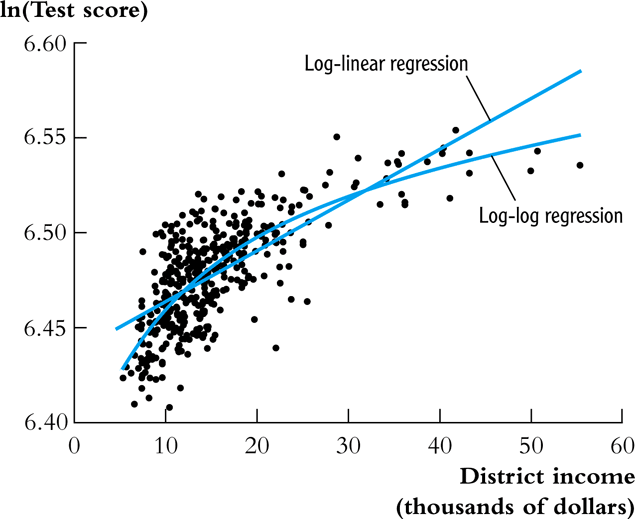
\includegraphics[width=0.65\textwidth]{img/fig-8-6.png}
\caption{\label{fig:org04cb59a}
The log-linear and log-log regression functions}
\end{figure}

\begin{table}[htbp]
\caption{Interpretation \(\beta_1\) in three logarithmic specifications}
\centering
\begin{tabular}{lp{4.5cm}p{8.5cm}}
Case & Regression specification & Interpretation of \(\beta_1\)\\
\hline
I & \(Y = \beta_0 + \beta_1 \ln(X) + u\) & A 1\% change in X is associated with a change in Y of \(0.01\beta_{1}\)\\
II & \(\ln(Y) = \beta_0 + \beta_1 X + u\) & A change in X by one unit is associated with a \(100\beta_1\%\) change in Y\\
III & \(\ln(Y) = \beta_0 + \beta_1 \ln(X) + u\) & A 1\% change in X is associated with a \(\beta_{1}\%\) change in Y, so \(\beta_1\) is the elasticity of Y with respect to X\\
\end{tabular}
\end{table}
\end{itemize}


\section{Interactions between independent variables}
\label{sec:orga725be1}

\subsection{Interactions between two binary variables}
\label{sec:org19d82d6}

\subsubsection*{The regression model with interaction between two binary variables}
\label{sec:orgebf3d1a}

Consider the population regression of earnings (\(Y_i\), where \(Y_i =
Earnings_i\)) against two binary variables: a worker has a college
degree (\(D_i\), where \(D_{1i} = 1\) if the i\(^{\text{th}}\) person graduated from
college) and a worker's gender (\(D_{2i}\), where \(D_{2i} = 1\) if the
i\(^{\text{th}}\) person is female).

Then the population regression model with an interaction term of
two binary variables is
\begin{equation}
\label{eq:interact-dd}
Y_i = \beta_0 + \beta_1 D_{1i} + \beta_2 D_{2i} + \beta_3 (D_{1i} \times D_{2i}) + u_i
\end{equation}
in which \(D_{1i} \times D_{2i}\) is the \textbf{interaction term}.

\subsubsection*{The method of interpreting coefficients in regressions with interacted binary variables}
\label{sec:org9debe52}
We follow a general rule for interpreting coefficients in Equation
(\ref{eq:interact-dd}):
\begin{quote}
First compute the expected values of \(Y\) for each possible case
described by the set of binary variables. Next compare these expected
values. Each coefficient can then be expressed either as an expected
value or as the difference between two or more expected values.
\end{quote}

\begin{itemize}
\item \textbf{Compute the expected values of \(Y\) for each possible combinations of \(D_1\) and \(D_2\)}
\label{sec:org00e8688}

\begin{description}
\item[{Case 1}] \(E(Y_i | D_{1i} = 0, D_{2i} = 0) = \beta_0\): the average
income of male non-college graduates is \(\beta_0\).
\item[{Case 2}] \(E(Y_i | D_{1i} = 1, D_{2i} = 0) = \beta_0 + \beta_1\): the
average income male college graduates is \(\beta_0 +
            \beta_1\).
\item[{Case 3}] \(E(Y_i | D_{1i} = 0, D_{2i} = 1) = \beta_0 + \beta_2\): the
average income of female non-college graduates is
\(\beta_0 + \beta_2\).
\item[{Case 4}] \(E(Y_i | D_{1i} = 1, D_{2i} = 1) = \beta_0 + \beta_1 +
            \beta_2 + \beta_3\): the average income of female college
graduates is \(\beta_0 + \beta_1 + \beta_2 + \beta_3\).
\end{description}

\item \textbf{Compute the difference between a pair of cases}
\label{sec:orga128804}

\begin{description}
\item[{Case 1 vs. Case 2}] \(E(Y_i | D_{1i} = 1, D_{2i} = 0) - E(Y_i |
     D_{1i} = 0, D_{2i} = 0) = \beta_1\). Thus, the average income
difference between college graduates and non-college graduates among
male workers is \(\beta\)\_1.
\item[{Case 1 vs. Case 3}] \(E(Y_i | D_{1i} = 0, D_{2i} = 1) - E(Y_i |
     D_{1i} = 0, D_{2i} = 0) = \beta_2\). Thus, the average income
difference between female and male workers who are not college
graduates is \(\beta_2\).
\item[{Case 1 vs. Case 4}] \(E(Y_i | D_{1i} = 1, D_{2i} = 1) - E(Y_i |
     D_{1i} = 0, D_{2i} = 0) = \beta_1 + \beta_2 + \beta_3\). Thus, The
average income difference between female college graduates and
male non-college graduates is \(\beta_1 + \beta_2 + \beta_3\).
\item[{Case 2 vs. Case 3}] \(E(Y_i | D_{1i} = 0, D_{2i} = 1) - E(Y_i |
     D_{1i} = 1, D_{2i} = 0) = \beta_2 - \beta_1\). Thus, the average
income difference between female non-college graduates and male
college graduates is \(\beta_2 - \beta_1\).
\item[{Case 2 vs. Case 4}] \(E(Y_i | D_{1i} = 1, D_{2i} = 1) - E(Y_i |
     D_{1i} = 1, D_{2i} = 0) = \beta_2 + \beta_3\). Thus, the average
income difference between female college graduates and male
college graduates is \(\beta_2 + \beta_3\).
\item[{Case 3 vs. Case 4}] \(E(Y_i | D_{1i} = 1, D_{2i} = 1) - E(Y_i |
     D_{1i} = 0, D_{2i} = 1) = \beta_1 + \beta_3\). Thus, the average
income difference between female college graduates and female
non-college graduates is \(\beta_1 + \beta_3\).
\end{description}

We can use t-statistic or F-statistic to test whether the differences
between different cases are statistically significant. For example, if
we want to test whether the average income of male college graduates
differs from that of male non-college graduates, the null hypothesis
is \(H_0: \beta_2 = 0 \text{ vs. } H_1: \beta_2 \neq 0\). Then, we can
use a t-statistic for this test. In another case, if we want to test
whether the average income of female college graduates differs from that
of female non-college graduates, the null hypothesis is \(H_0:
\beta_1 + \beta_3 = 0 \text{ vs. } H_1: \beta_1 + \beta_3 \neq
0\). Then, we need to use an F-statistic for this test.
\end{itemize}


\subsection{Interactions between a continuous and a binary variable}
\label{sec:org9ce99fe}
Consider the population regression of earnings (\(Y_i\)) against one
continuous variable, individual's years of work experience (\(X_i\)),
and one binary variable, whether the worker has a college degree
(\(D_i\), where \(D_i=1\) if the i\(^{\text{th}}\) person is a college graduate).

As shown in Figure \ref{fig:org6a9773e}, the population regression line relating \(Y\) and
\(X\) depends on \(D\) in three different ways.

\begin{figure}[htbp]
\centering
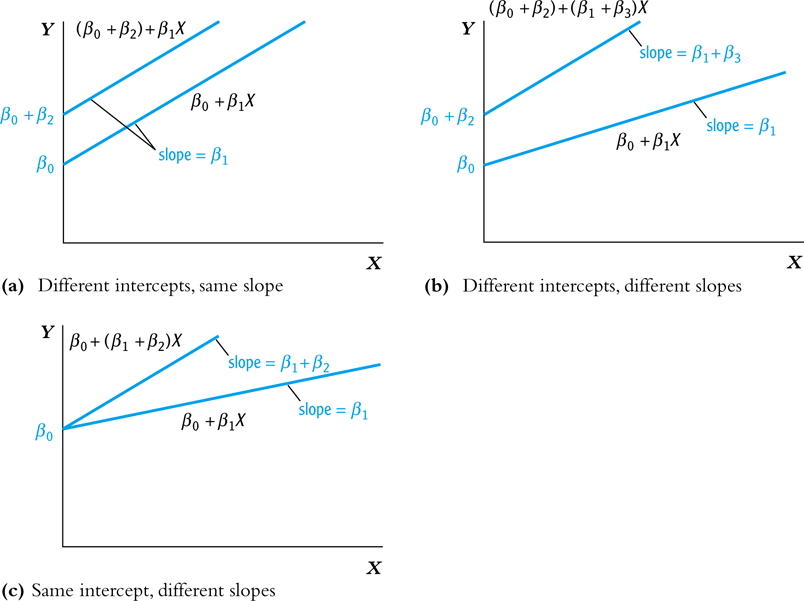
\includegraphics[width=0.95\textwidth]{img/fig-8-8.png}
\caption{\label{fig:org6a9773e}
Regression Functions Using Binary and Continuous Variables}
\end{figure}

\subsubsection*{Different intercept, same slope.}
\label{sec:orgfe4873f}
As shown in Figure \ref{fig:org6a9773e} (a), the corresponding population
regression model is
\begin{equation}
\label{eq:interact-dx-a}
Y_i = \beta_0 + \beta_1 X_i + \beta_2 D_i + u_i
\end{equation}

\begin{itemize}
\item From Equation (\ref{eq:interact-dx-a}), we have the population
regression functions as \(E(Y_i | D_i = 1) =
  \beta_0 + \beta_1 X_i + \beta_2\) and \(E(Y_i | D_i
  = 0) = \beta_0 + \beta_1 X_i\). Thus, \(E(Y_i | D_i = 1) - E(Y_i | D_i
  = 0) = \beta_2\).
\item The average initial salary of college graduates is higher than
non-college graduates by \(\beta_2\), and this gap persists at the same
magnitude regardless of how many years a worker has been working.
\end{itemize}

\subsubsection*{Different intercepts and different slopes.}
\label{sec:org360b9f7}
As shown in Figure \ref{fig:org6a9773e} (b), to allow for different slopes, we
need to add an interaction term to Equation (\ref{eq:interact-dx-a})
as follows:
\begin{equation}
\label{eq:interact-dx-b}
Y_i = \beta_0 + \beta_1 X_i + \beta_2 D_i + \beta_3 (X_i \times D_i) + u_i
\end{equation}

\begin{itemize}
\item The population regression functions for the two cases are
\(E(Y_i|D_i=1) = (\beta_0+\beta_2) + (\beta_1 + \beta_3) X_i\) and
\(E(Y_i|D_i=0) = \beta_0 + \beta_1 X_i\). Thus, \(\beta_2\) is the
difference in intercepts and \(\beta_3\) is the difference in slopes.
\item The average initial salary of college graduates is higher than
non-college graduates by \(\beta_2\), and this gap will widen (or
narrow) depending on the effect of the years of work experience on
earnings.
\end{itemize}

\subsubsection*{Different intercepts and same intercept.}
\label{sec:org6c3cc9b}
As shown in Figure \ref{fig:org6a9773e} (c), there is no difference in the
intercept between the two regression line, but they have different
slopes. The corresponding regression model is
\begin{equation}
\label{eq:interact-dx-c}
Y_i = \beta_0 + \beta_1 X_i + \beta_2 (X_i \times D_i) + u_i
\end{equation}

\subsection{Interactions between two continuous variables}
\label{sec:org0e7363b}
Now we consider the regression of earnings against two continuous
variables, one for the years of work experience (\(X_1\)) and another
for the years of schooling (\(X_2\)). The interaction term \(X_{1i}
\times X_{2i}\) can be included to account for (1) the effect of
working experience on earnings, depending on the years of schooling,
and (2) conversely, the effect of the years of schooling on earnings,
depending on working experience.

The regression model with the interaction between \(X_1\) and \(X_2\) is
\begin{equation}
\label{eq:interact-xx}
Y_i = \beta_0 + \beta_1 X_{1i} + \beta_2 X_{2i} + \beta_3 (X_{1i} \times X_{2i}) + u_i
\end{equation}

\begin{itemize}
\item The effect of a change in \(X_1\), holding \(X_2\) constant, is
\[ \frac{\partial Y}{\partial X_1} = \beta_1 + \beta_3 X_2 \text{ for
  continuous variables} \]
or generally,
\[ \frac{\Delta Y}{\Delta X_1} = \beta_1 + \beta_3 X_2 \]
\item Similarly, the effect of a change in \(X_2\), holding \(X_1\) constant, is
\[ \frac{\Delta Y}{\Delta X_2} = \beta_1 + \beta_3 X_1 \]
\end{itemize}

\section{Regression Functions That Are Nonlinear in the Parameters}
\label{sec:orgf1d66fc}

All the regression models that we have discussed in this lecture are
nonlinear in the regressors but linear in parameters so that we can
still treat them as linear regression models and estimate using the
OLS. However, there exist regression models that are nonlinear in
parameters. For these models, we can either transform them to the
"linear" type of models or estimate using the \textbf{nonlinear least
squares} (NLS) estimators.

\subsection{Transform a nonlinear model to a linear one}
\label{sec:orgbd4ab50}

Suppose we have a nonlinear regression model as follows
\begin{equation}
\label{eq:nls-xaxb}
Y_i =  \alpha X_{1i}^{\beta_1}X_{2i}^{\beta_2}\cdots X_{ki}^{\beta_k}e^{u_i}
\end{equation}
which is nonlinear in both \(X\) and \(\beta\). The Cobb-Douglas utility
(or production) function takes the form as in Equation
(\ref{eq:nls-xaxb}).

Although Equation (\ref{eq:nls-xaxb}) is nonlinear in \(\beta\), we can
easily transform it to be linear in \(\beta\) by taking the natural
logarithmic function on both sides of the equation, yielding the
following equation:
\begin{equation}
\label{eq:nls-linear-xaxb}
\ln(Y_i) = \ln(\alpha) + \beta_1 \ln(X_{1i}) + \beta_2 \ln(X_{2i}) + \cdots + \beta_k \ln(X_{ki}) + u_i
\end{equation}
Let \(\beta_0 = \ln(\alpha)\). Equation (\ref{eq:nls-xaxb}) becomes a
log-log regression model, which is linear in all parameters and can be
estimated using the OLS. \(\beta_i\) for \(i=1, 2, \ldots, k\) are the
elasticities of \(Y\) with respect to \(X_i\).

\subsection{Nonlinear models that cannot be linearized}
\label{sec:org7b19ec5}

There are nonlinear models that cannot be linearized by any
transformation. We introduce two examples.

\subsubsection*{Logistic curve}
\label{sec:org6e64c46}

Sometimes we may have a dependent variable taking values between 0 and
1, such as the fraction of students who get the test scores lower
than 70. The linear regression model generally cannot guarantee the
predicted dependent variable to be bounded between 0 and 1. For this
reason, we can use the logistic function to set up a nonlinear
regression function.

The logistic regression model with k regressors is
\begin{equation}
\label{eq:logistic}
Y_i = \frac{1}{1 + \exp(\beta_0 + \beta_1 X_{1i} + \cdots \beta_k X_{ki})} + u_i
\end{equation}

The logistic function with a single \(X\) is graphed in Figure \ref{fig:org8679f3e}(a). The
logistic function has an elongated "S" shape.
\begin{itemize}
\item For small values of \(X\), the value of the function is nearly 0 and
the shape is flat.
\item For large values of \(X\), the function approaches 1 and the slope is
flat again.
\end{itemize}

\subsubsection*{Negative exponential growth function}
\label{sec:org7ee47fa}

Sometimes the effect of \(X\) on \(Y\) must be positive and the effect is
bounded by a upper bound. For this case, we can use a negative
exponential growth function to set up a regression model as follows
\begin{equation}
\label{eq:neg-exp}
Y_i = \beta_0 [1-\exp(-\beta_1(X_i - \beta_2))] + u_i
\end{equation}

The negative exponential growth function is graphed in Figure
\ref{fig:org8679f3e}(b), which has the desired properties:
\begin{itemize}
\item The slope is positive for all values of \(X\).
\item The slope is greatest at low values of \(X\) and decreases as \(X\)
increases.
\item There is an upper bound, that is, a limit of \(Y\) as \(X\) goes to
infinity, \(\beta_0\).
\end{itemize}

\begin{figure}[htbp]
\centering
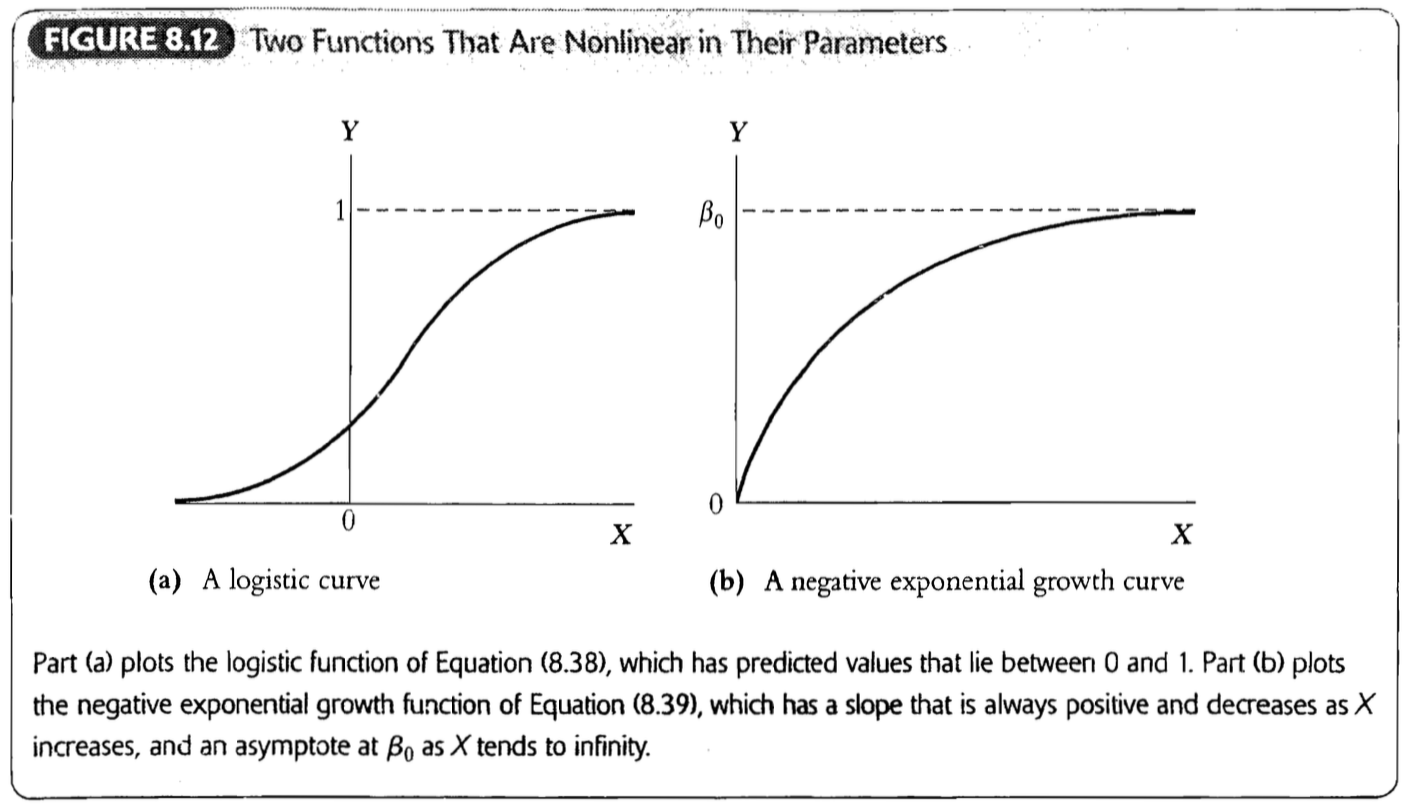
\includegraphics[width=.9\linewidth]{img/fig-8-12.png}
\caption{\label{fig:org8679f3e}
The logistic and negative exponential growth functions}
\end{figure}

\subsubsection*{The nonlinear least squares estimators}
\label{sec:org8bbad12}
For a nonlinear regression function
\[ Y_i = f(X_1, \ldots, X_k; \beta_1, \ldots, \beta_m) + u_i \]
which is nonlinear in both \(X\) and \(\beta\), we can obtain the
estimated parameters by \textbf{nonlinear least squares} (NLS) estimation. The
essential idea of NLS is the same as OLS, which is to minimize the sum
of squared prediction mistakes. That is
\begin{equation*}
\operatorname*{min}_{b_1, \ldots, b_m}\: S(b_1, \ldots, b_m) = \sum_{i=1}^n \left[ Y_i - f(X_1, \ldots, X_k; b_1, \ldots, b_m) \right]^2
\end{equation*}
The solution to this minimization problem is the nonlinear least
squares estimators.
\end{document}